\documentclass{article}

\usepackage{graphicx}
\usepackage{array}
\usepackage[group-separator={,}]{siunitx}
\usepackage{authblk}	% prettier multiple authors

\usepackage{tikz}

\usepackage{hyperref}

% see http://texblog.org/2008/05/07/fwd-equal-cell-width-right-and-centre-aligned-content/
\newcolumntype{x}[1]{%
>{\centering\hspace{0pt}}p{#1}}%


\title{Real Time Social Data Sampling }
\author[]{Scott Hendrickson}
\author[]{Brian Lehman}
\author[]{Joshua Montague}
\affil[]{ \Large{Gnip, Inc.} }

\begin{document}
\maketitle

%%%%%%%%%%%%%%%%%%%%%%%%%%%%%%%%%%
\section{Introduction}

We often wish to calculate social activity rates to identify signals of emerging topics or stories.
We want to know what we can detect and understand the certainty of our estimates. This means
we need to calculate the relationship between activity counts, signal sensitivity and confidence. This
is illustrated in Figure~\ref{fig:tradeoff}. The event rate is the number of activities per time,
the signal is the change in rate, and confidence comes from the statistics of the activities and
sampling operators. Time enters the calculation because the longer we count, the more activities
we count.

%%%%%
% simplest figure
%
%\begin{figure}[h]
%\begin{center}
%\begin{tikzpicture}
%\draw (0,0) node[anchor=north]{activities}-- (1.5,2.598)node[anchor=south]{signal} -- (3,0)node[anchor=north]{confidence}-- (0,0);
%\end{tikzpicture}
%\end{center}
%\caption{The number of events is a product of the rate and time. Signal is
%the change in event rate we want to detect. Confidence characterizes the uncertainty
%in our estimate of rate. These parameters are not independent: choose any two and
%calculate the third. }
%\label{fig:tradeoff}
%\end{figure}
%
%
%%%%%

%%%%%
% figure
%
\begin{figure}[h]
\begin{center}
	%%%%%
	%
	% http://cremeronline.com/LaTeX/minimaltikz.pdf
	%
	%%%%%
	% Python generate arrows
	%	import math
	%	a=.5*math.sin(2.*math.pi/6)
	%	b=.5*math.cos(2.*math.pi/6)
	%	h=3.*math.sin(2.*math.pi/6)
	%	a1 = (b,a)
	%	a2 = (0.5,0)
	%	b1 = (1.5 - b, h - a)
	%	b2 = (1.5 + b, h - a)
	%	c1 = (3-b,a)
	%	c2 = (3-0.5,0)
	%	print "\draw [thick, <->]",a1,"--",b1,";"
	%	print "\draw [thick, <->]",b2,"--",c1,";"
	%	print "\draw [thick, <->]",c2,"--",a2,";"
	%%%%% 
	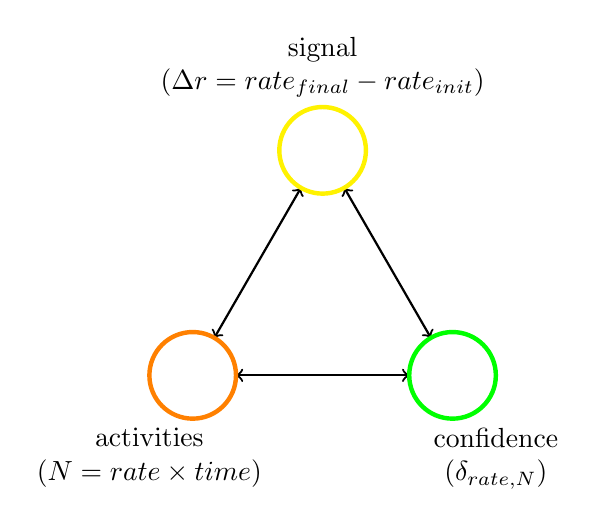
\begin{tikzpicture}[scale=1.1]]
	% arrows
	\draw [thick, <->] (0.25000000000000006, 0.4330127018922193) -- (1.25, 2.165063509461097) ;
	\draw [thick, <->] (1.75, 2.165063509461097) -- (2.75, 0.4330127018922193) ;
	\draw [thick, <->] (2.5, 0) -- (0.5, 0) ;
	% circles
	\draw [orange, ultra thick] (0,0) circle [radius=0.5];
	\draw [yellow, ultra thick] (1.5,2.598) circle [radius=0.5];
	\draw [green, ultra thick] (3,0) circle [radius=0.5];
	% labels
	\node[align=center, below] at (-0.5,-0.5){activities\\($N=rate \times time$)};
	\node[align=center, above] at (1.5,3.098){signal\\($\Delta r=rate_{final}-rate_{init}$)};
	\node[align=center, below] at (3.5,-0.5){confidence\\($\delta_{rate,N}$)};
	\end{tikzpicture}
\end{center}
\caption{The number of activities is a product of the rate and time. Signal is
the change in event rate we want to detect. Confidence characterizes the uncertainty
in our estimate of rate. These parameters are not independent: choose any two and
calculate the third. }
\label{fig:tradeoff}
\end{figure}
%
%
%%%%%

%%%%%
% hand drawn figure
%
%\begin{figure}[h]
%    	%\centering
%	\begin{center}
%		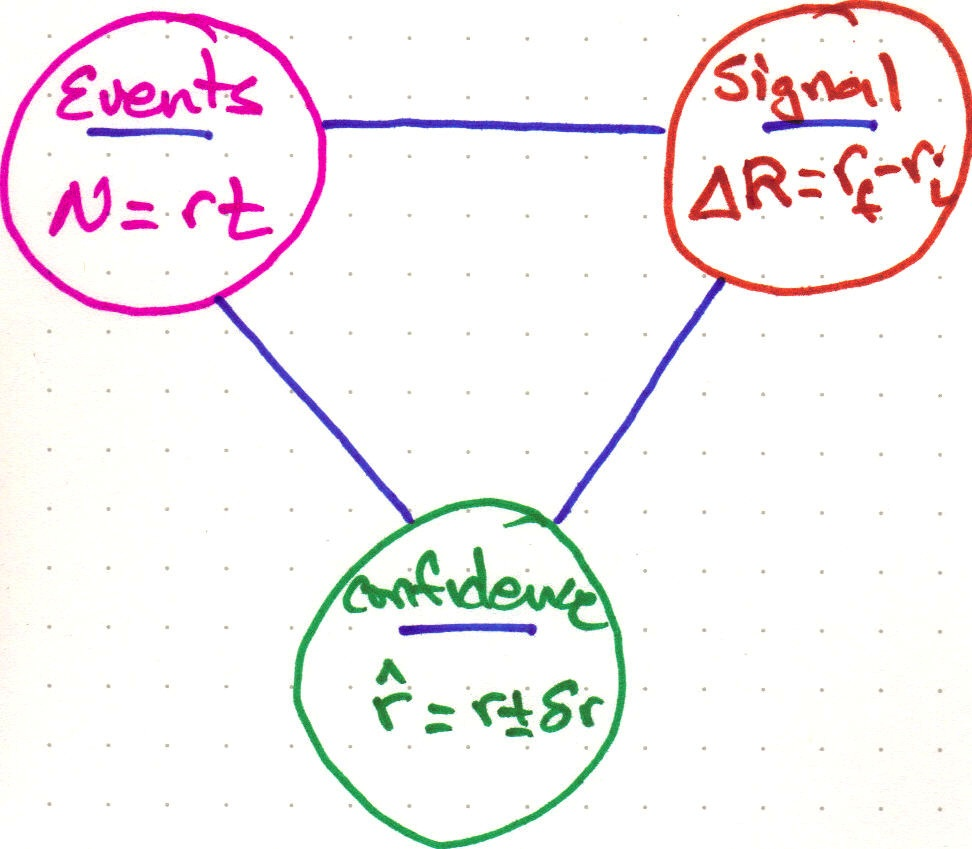
\includegraphics[width=1.75in]{./imgs/tradeoff.jpg}
%	\end{center}
%\caption{The number of events is a product of the rate and time. Signal is
%the change in event rate we want to detect. Confidence characterizes the uncertainty
%in our estimate of rate. These parameters are not independent: choose any two and
%calculate the third. }
%\label{fig:tradeoff}
%
%
%%%%%

For many topics, social media streams contain data with sufficient frequency to create reliable, high-resolution signals in short observation times.  But for the less common topics, the activities (e.g. blog posts or tweets) are less frequent and we need to take care in identifying the observation time, signal sensitivity and confidence level. These three quantities are related; typically, we can choose two and calculate the third.

There are a handful of related questions that may come up regarding sampling and signals.  In the next section, we list some of these questions to explore the meaning of the relationships outlined above. After that, we will look at filtering and sampling in a little more detail.  The middle of this white paper builds up the calculation method required to answer these questions. Finally, in the last section, we provide example calculations.

%%%%%%%%%%%%%%%%%%%%%%%%%%%%%%%%%%
\subsection{Motivating Questions} 

Common questions regardind rate, signal and confidence level:

\begin{itemize}
	\item The activity rate has doubled from five counts to ten counts between two of my buckets. Is this a significant change? 
	Or is this expected variation due to low-frequency events?
	\item I want to minimize the total number activities I consume, what sampling factor should I use if I want to detect
	changes of 2x in activity rate in 1-hour?
	\item How long should I observe and count activities to detect a change in signal of 5\%?
	\item How do I describe the trade-off between signal latency (how long I have to wait) and rate uncertainty (how 
	confidently I can estimate activity rate)?
	\item How do I define confidence levels on rate estimates for a social activity time series with only 20 events per day?
	\item I plan to bucket the data in order to estimate activity rate, how big (i.e. what duration) should the buckets be? 
	\item How many activities should I target to collect in each bucket in order to be have a 95\% confidence that my 
	rate estimate is accurate for each bucket? 
%\item \ldots
\end{itemize}

%%%%%%%%%%%%%%%%%%%%%%%%%%%%%%%%%%
\subsection{Sample Operators and Order of Filters} 

In order to to control costs or to scale analysis, we may choose to sample a known fraction of the total social activities. This presents an
additional complexity to the ideas introduced in the introduction. Using a sampling filter effectively decreases the rate of activities. If you
plan to use a sampling filter, it may be useful to explore sampling before moving the the core of the calculation.  
If not, please skip to the next section.

There are two approaches to sampling a firehose of social data. Both involve reducing the number of activities in the 
real time stream to a manageable size for analysis. \footnote{Twitter's filtered, rate-limited 1\% streaming API provides a 
non-deterministic combination that is not suitable for many analytic tasks.  See \cite{Morstatter:2013}.} 

The first step is to use keyword filtering.  Gnip provides filtering on keywords to select only the portion of the stream
that is relevant to the topic you want to analyze. For example, if you are interested in tracking the Super Bowl, you 
might start with a broad stream defined by the keywords ``superbowl" ``super~bowl" and ``contains:xlvii", the 
latter being the Roman numeral of the Super Bowl as might be seen in hashtags or short links. This would limit the 
social data stream to activities related to the Super Bowl.

In the case of a major event like the Super Bowl, the keyword-filtered stream may represent a very large number
of activities.  In this case, a second step might be to filter this stream to a known fraction of the total firehose. For 
example, using Gnip's sampling operator, we can reduce the stream to only fraction, e.g. 12\%, of the activities. 
The corresponding Powertrack rule would become  ``(super bowl OR superbowl) sample:12''.

It is useful to know how Gnip's sampling algorithms work to inform sampling decisions.  Sampling is available on
Gnip's premium streams including Tumblr, Twitter, Wordpress and Disqus. Some key features of Gnip sampling:

\begin{enumerate}
	\item 1\% resolution
	\item Stable sampling rate (short time resolution)
	\item Sample is deterministic and returns the same activites for near-rule matches.  For example, this means
	that you will get the same tweets for matches to the ``super bowl'' portion of the rules ``super bowl sample:12'' 
	and ``(super bowl OR superbowl) sample:12''
	\item Sampling is progressively inclusive (i.e. a 2\% stream (e.g. ``sample:2'') includes the exact activities from
	the 1\% stream plus an 
	additional 1\%,  and so on)
	\item Activities are first selected from the firehose to reach the desired sampling rate and then filtered by keywords 
\end{enumerate}

What happens when we look at the combination of filtering with sampling?  Continuing with our Super Bowl example, 
assume our term filtering rules return $y=5\%$ of the stream. Assume further that we sample $x=12\%$ sample of 
the firehose activities and the total activities for the day are $N_f=500$M. Filtering and sampling will leave us with 
approximately,

\begin{equation}
    \label{eq:sbsample}
    N_{observed} = x y N_{firehose}= 0.12 (0.05) 500 \textrm{ M} = 3 \textrm{ M}
\end{equation}
activities in a day. 

Once you understand this order, it is natural to ask why Gnip does not filter first, then sample. The difference is not
in the final outcome, but how long you have to wait for a reliable estimate of rate. If Gnip were to filter on keywords
first, Equation~\ref{eq:sbsample} would also be a reasonable estimate of $N_{observed}$ on the time scale of the 
sampling calculation. However, this process would require relaxing properties 3 and 4 in the list above. Both attributes
are desirable for most social data projects. Doing the sample first, followed by the keyword filter, gives a slightly
more complex behavior because it requires us to deal the effects of statistical variations in the short term.

%%%%%%%%%%%%%%%%%%%%%%%%%%%%%%%%%%%%%%%%%%%%%%%%%%%%%%%%%%%%%%%%%%%
\section{Signal} 

In many situations, the main question is: \emph{``How many events must we observe in order to detect a change in activity rate?"} Answering
this question requires an understanding of the trade offs between sampling time, activity rates, and signal size.  First, 
we will define signal in terms of the activity rate.

%%%%%%%%%%%%%%%%%%%%%%%%%%%%%%%%%%
\subsection{Activity Rate} 

The average activity rate is calculated by,

\begin{equation}
    \label{eq:rateEst}
    \bar{r} = \frac{N}{T}
\end{equation}
where $N$ is the number of activities and $T$ the time period over which we count activities.  Because there will be statistical
variations in the number of activities in any given time interval, there will be some uncertainty in our estimate of average rate. 
The more activities we count, the lower the uncertainty in our estimate as shown in Figure~\ref{fig:confidence}.

%%%%%
% figure
%
\begin{figure}[h]
	\begin{center}
		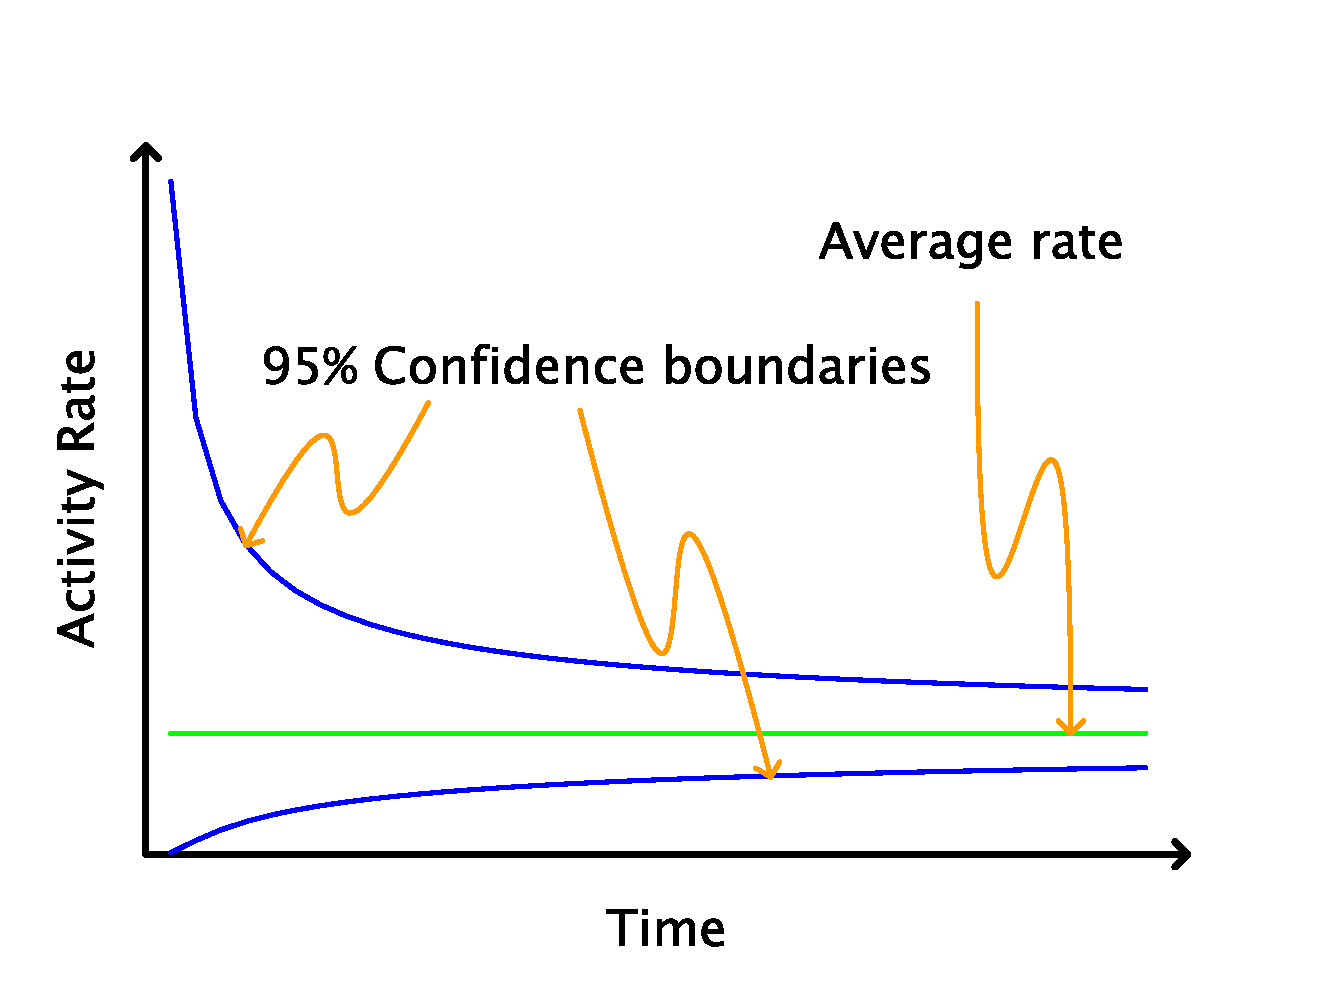
\includegraphics[width=3.5in]{./imgs/fig2.pdf}
	\end{center}
	\caption{Uncertainty in the estimated rate of activities goes down as we wait longer in order to count more activities.  The green line
represents the rate while the blue lines show the upper and lower 95\% confidence band. }
    	\label{fig:confidence}
\end{figure}
%
%
%%%%%

Below, we will determine how many activities $N$ we need to count to estimate the average activity rate, $\bar{r}$, to a desired level
of confidence (e.g. 95\%). Or, inverting this question: given a level of confidence, how wide is the range of uncertainty
about the rate estimate?

The details of calculating the confidence level can be found in the next section.  Next, we explore the connection between
uncertainty in the rate estimate and the size of the signal we can detect.

%
% Add shaded version of fig 1 to show what we are working on now?
%

%%%%%%%%%%%%%%%%%%%%%%%%%%%%%%%%%%
\subsection{Signal Sensitivity}

When activity rates are high, rate estimates will be more certain; when low, rate estimates will be less certain. High uncertainty
in the rate estimates may hide the small changes in activity rates we wish to identify.  The variation in activity rate due to the statistics
associate with infrequent events (or short observation time) must be smaller than the signal we want to detect. Therefore, we observe
a valid signal in a time series when the activity rate has changed by more than the rate signal sensitivity, $\Delta r$, defined as,

\begin{equation}
    \label{eq:signal}
    | r(t_f) - r(t_i) | \geq \Delta r.
\end{equation}

The associated time scale of the change, $T_l = t_f - t_i$, is the signal latency.  This definition implies that we 
must observe activities for a time, $T > T_l$, to achieve the desired signal sensitivity, $\Delta r$.

%%%%%
% figure
%
\begin{figure}[h]
    \centering
    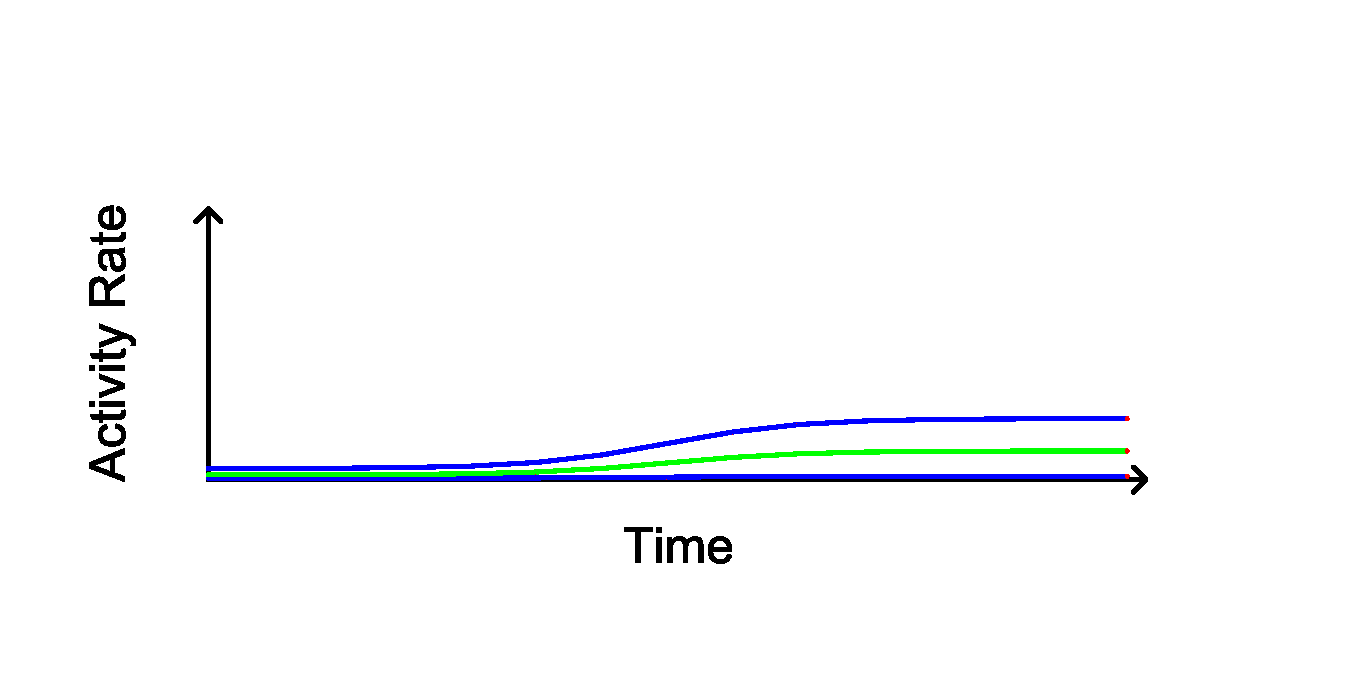
\includegraphics[width=3.5in]{./imgs/fig3a.pdf}
    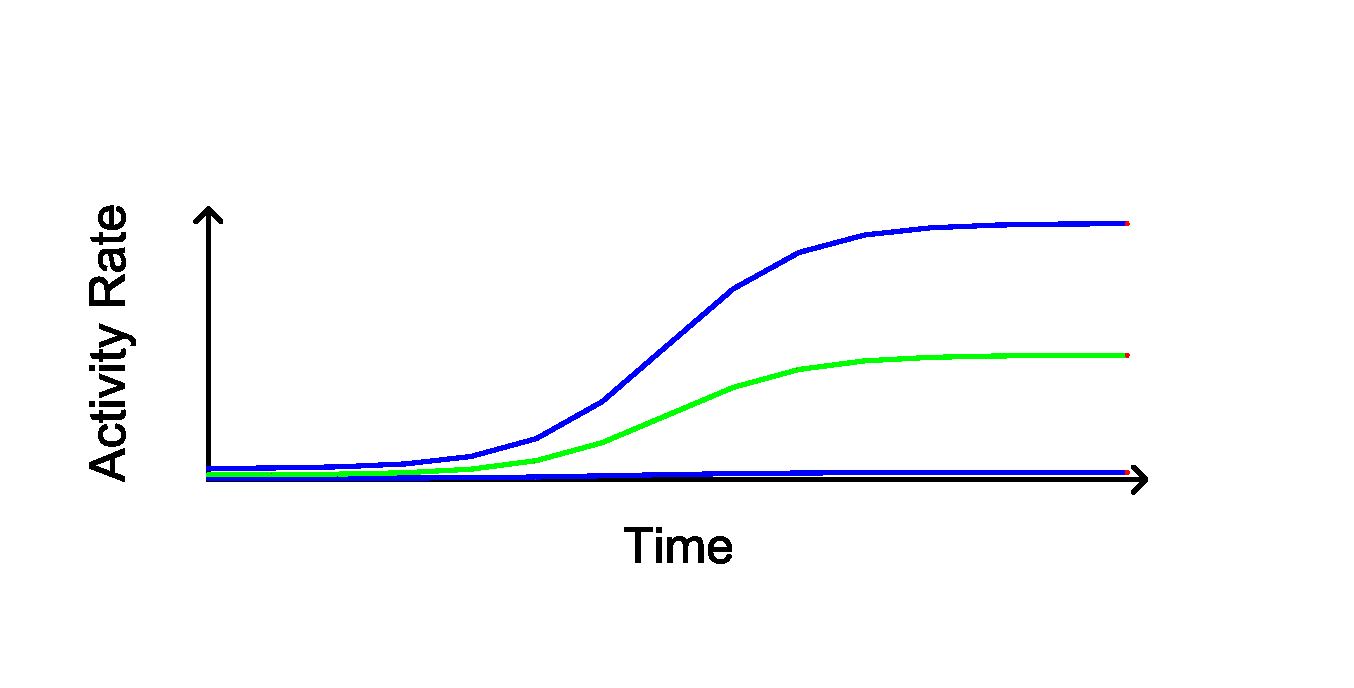
\includegraphics[width=3.5in]{./imgs/fig3b.pdf}
        \caption{A signal can be detected when the change in rate is greater than the uncertainty in the rate estimates.}
    \label{fig:signal}
\end{figure}
%
%
%%%%%

%%%%%%%%%%%%%%%%%%%%%%%%%%%%%%%%%%
\subsection{Signal Sensitivity--Confidence Criteria} 

We will be estimating the activity rate in Equation~\ref{eq:rateEst} by counting activities for a determined time period.  The
number activities in any given period will be distributed about the long term mean. As we count more activities, our
estimate of rate will converge toward the true value.  If we count thousands of activities per minute, our confidence of the estimate
of activity rate will be very high after a short time.  For rare activities, we will have to count longer before we have
a high level of confidence in our rate estimate.

Referring to the signal sensitivity definition in Equation~\ref{eq:signal}, we can establish a rough criteria for confidence
in terms of signal uncertainty, $\delta r$:

\begin{equation}
    \label{eq:criteria}
    \frac{\delta r}{\bar{r}_{max}} << \frac{\Delta r}{\bar{r}_{max}}.
\end{equation}
where $\bar{r}_{max}$ will be the lower rate estimate (initial if detecting rising activity rate but final if detecting falling activity rate).

To help quantify this inequality, we introduce a criteria factor, $\eta$, that tells how much larger than the relative
uncertainty the change in rate must be.

\begin{equation}
    \label{eq:criteriaParam}
    \frac{\delta r}{\bar{r}_{max}} = \frac{\eta \Delta r}{\bar{r}_{max}}
\end{equation}
where $\eta \ge 1$.

This criteria represents the trade off between signal size and confidence.

%%%%%%%%%%%%%%%%%%%%%%%%%%%%%%%%%%%%%%%%%%%%%%%%%%%%%%%%%%%%%%%%%%%
\section{Statistics of Time Series of Activities} 

In this section, we examine the underlying statistics in order to calculate confidence intervals and confidence levels.

%%%%%%%%%%%%%%%%%%%%%%%%%%%%%%%%%%
\subsection{Poisson Activity Probability} 

A model of counts of rare activities is that the inter-arrival times are exponentially distributed, 

\begin{equation}
    \label{eq:tbe}
    p_{activity}(t) = r e^{-r t}
\end{equation}

This assumption leads to a Poisson distribution of activity counts over time.

The probability of observing $n$ activities in time $t$ when the activity rate is $r$ is given by,
\begin{equation}
    \label{eq:poisson}
    P(n) = \frac{e^{-r t} (r t)^n}{n!}
\end{equation}

The expected value is $E[n]=n=rt$. The mean and variance of the Poisson distribution are both equal to $r$.

%%%%%%%%%%%%%%%%%%%%%%%%%%%%%%%%%%
\subsection{Poisson Confidence Intervals} 

We are counting activities in a defined time interval to estimate the activity rate $\bar{r}$. Confidence intervals \cite{Geo2012} for the
Poisson distribution with confidence level $\text{conf\%} = 100\%(1-\alpha)$ are given by,

\begin{equation}
    \label{eq:chisqconf}
    \frac{1}{2T} \chi^2(\alpha/2;2n) \leq r \leq \frac{1}{2T} \chi^2(1-\alpha/2;2n+2)
\end{equation}
where $\chi^2$ is the inverse cumulative distribution function, $CDF^{-1}(p; n)$, of the $\chi^2$ distribution.\footnote{A useful approximation to the exact interval is given by  $[ n(1 - \frac{1}{9n} - \frac{z_{\alpha}}{3\sqrt{n}})^3 , (n+1)(1- \frac{1}{9(n+1)} + \frac{z_{\alpha}}{3\sqrt{n+1}})^3]$. }
Note that with this definition of $\alpha$, a confidence interval of 90\% corresponds to $\alpha=0.1$.

Confidence interval sizes for confidence levels of 90\% are shown in Table \ref{tab:conf}

\begin{table}\centering
    \begin{tabular}{r|x{3.5cm}|r|r}
     \hline
N & Interval Bounds & Interval Size ($\delta n$) & Relative Interval\\ 
\hline 
1 &   0.0513, 4.744  & 4.693 & 4.693\tabularnewline 
2 &   0.3554, 6.296  & 5.940 & 2.970\tabularnewline 
3 &   0.8177, 7.754  & 6.936 & 2.312\tabularnewline 
4 &   1.366, 9.154  & 7.787 & 1.947\tabularnewline 
5 &   1.970, 10.51  & 8.543 & 1.709\tabularnewline 
6 &   2.613, 11.84  & 9.229 & 1.538\tabularnewline 
7 &   3.285, 13.15  & 9.863 & 1.409\tabularnewline 
8 &   3.981, 14.43  & 10.45 & 1.307\tabularnewline 
9 &   4.695, 15.71  & 11.01 & 1.223\tabularnewline 
10 &   5.426, 16.96  & 11.54 & 1.154\tabularnewline 
20 &   13.25, 29.06  & 15.81 & 0.7904\tabularnewline 
30 &  21.59, 40.69  & 19.10 & 0.6366\tabularnewline 
40 &  30.20, 52.07  & 21.87 & 0.5468\tabularnewline 
50 &  38.96, 63.29  & 24.32 & 0.4864\tabularnewline 
60 &  47.85, 74.39  & 26.54 & 0.4423\tabularnewline 
70 &  56.83, 85.40  & 28.57 & 0.4082\tabularnewline 
80 &  65.88, 96.35  & 30.47 & 0.3809\tabularnewline 
90 &  74.98, 107.2  & 32.25 & 0.3584\tabularnewline 
100 &  84.14, 118.1  & 33.94 & 0.3394\tabularnewline 
200 &  177.3, 224.9  & 47.55 & 0.2378\tabularnewline 
300 &  272.1, 330.1  & 58.00 & 0.1933\tabularnewline 
400 &  367.7, 434.5  & 66.82 & 0.1670\tabularnewline 
500 &  463.8, 538.4  & 74.58 & 0.1492\tabularnewline 
750 &  705.5, 796.6  & 91.11 & 0.1215\tabularnewline 
1000 &  948.6,  1054.  & 105.0 & 0.1050\tabularnewline 
\end{tabular}
\caption{Confidence intervals given the number of events counted $N$ in unit time $T$.  Rate interval 
size is $\delta r = \delta N/T$. Note that the relative uncertainty goes down while the absolute size of the interval increases.}
\label{tab:conf}
\end{table}

To determine the parameters satisfying our data collection goals, we find the value of $n$ for which
the time interval and confidence level match our requirements for signal detection.  That is, we can
now calculate any one of signal sensitivity, signal latency, activity rate, and confidence level given
the other parameters. Calculations for various design choices are illustrated in the last section of this paper.

%%%%%%%%%%%%%%%%%%%%%%%%%%%%%%%%%%
\subsection{Confidence Interval Approximations and Bucketed Activity Counts}

This section deals with approximations to the Poisson confidence interval for large numbers of activities. In
addition, we it contains some observations about bucketed activity counts. You can skip this section and
move to calculations if these ideas don't apply to your system.

\subsubsection{Frequent Activities} 

When we observe large numbers of activities, the confidence interval can be estimated using the Normal
approximation. For example, for $95\%$ confidence interval the interval is symmetric about the mean
and given by,

\begin{equation}
    \label{eq:largenconf}
    \bar{r} - 1.96 \sqrt{\bar{r}/n} \leq \hat{r} \leq \bar{r} + 1.96 \sqrt{\bar{r}/n}
\end{equation}

\subsubsection{Bucketed Activity Counts}

For many reasons, counts may be collected in buckets of some pre-defined time length.  The rate information
may by more naturally calculated by bucket rather than the total time $T$ required by our confidence
requirements. In general, define the relationship between $T$ and the bucket size (constant) as,

\begin{equation}
    \label{eq:bucket}
    \Delta t = \frac{T}{k}
\end{equation}
where $k$ is the number of buckets that we need to aggregate to observe for time $T$. This parameter
can be used to calculate a corresponding signal latency, $k_l = T_l/\Delta t$.

Resolution times are interchangeable with number of buckets $k$ given $\Delta t << T$.  In general, the
bucket resolution time will not be an even multiple of the bucket size.  In this case, imposing the calculation
of average rate per bucket $\bar{r} = n/\Delta t$ adds another layer of variability.

%%%%%%%%%%%%%%%%%%%%%%%%%%%%%%%%%%
\subsection{Summary of Parameters and Trade offs}

When activities are common, we can estimate the activity rate to a high level of certainty in a short time. With lower
uncertainty in our estimate of activity rate, we can detect small changes in activity rate--we have high Signal
Sensitivity. For rare activities, we have to wait longer to count enough activities to estimate the activity rate to
the desired level of confidence to detect a small signal. These trade offs are summarized in the Table~\ref{tab:tradeoff}.

For reference, we assemble the parameter definitions and a table summarizing trade offs.  Table~\ref{tab:summary}
summarizes the parameters of the model. Table~\ref{tab:tradeoff} summarizes the trade offs in parameters for
a given target.

\begin{table} [!h]
    \begin{tabular}{p{3.0cm}| p{1.9cm}|p{5.9cm}}
     \hline
Parameter  & Symbol & Definition \\
\hline	
Activity count & $N$ & Number of activities in time $T$\\
Sample time & $T$	& Duration of observation\\
Activity rate & $r$	& Number of activities per time $T$\\
Avg. activity rate & $\bar{r} = N/T$ & Our estimate of average activity rate \\
Rate variability & $\delta r$	& Uncertainty of rate estimate \\
Confidence & $\alpha$ & Confidence level is $1-\alpha$\\
Signal sensitivity & $\Delta r=r_{f}-r_{i}$ & Detectable change in activity rate \\
Signal latency & $T_l$ & Time required to detect $\Delta r$  \\
Signal confidence & $\eta$ & Rate signal criteria multiplier factor (i.e. $\eta = 3$ means relative signal is $3 \times$ random variations in sample) \\
Bucket & $\Delta t$ & Predetermined time scale for estimating rate (probably already determined in your system)\\
Number of buckets & $k=T/\Delta t$ & Duration expressed in number of  buckets \\
Sampling rate & $S$	& Powertrack sampling operator (e.g. ``sample:$S$'') \\
\hline
\end{tabular}
\caption{Summary of model parameters.}
\label{tab:summary}
\end{table}

\begin{table}[!h]
    \begin{tabular}{ p{3.0cm}| p{5.2cm} | p{2.6cm}}
     \hline
Goal  & Possible Actions & Example\\
\hline
Minimize activities (i.e. decrease $N$)  & increase $\Delta r$ (decrease signal sensitivity); decrease 
	confidence (E.g. from 95\% to 90\% ); increase $T_l$ (wait longer for the signal)  & See example 
	in Section \ref{ex:1} that illustrates long signal latency\\
\hline	
Increase signal sensitivity (i.e. decrease $\Delta r$) & increase $T$ (increase number of buckets ($k$); 
	increase bucket size ($\Delta t$) ); increase activity rate ($r$) by broadening filter or increase 
	Powertrack sampling  & See example in Section \ref{ex:3} that illustrates sensitivity with high rate\\
\hline
Decrease signal latency  (i.e. decrease $T_l$)   & decrease signal sensitivity $\Delta r$;
	decrease confidence factor ($\alpha$); increase activity rate ($r$) by broadening filter 
	or increase Powertrack sampling  & See example in Section \ref{ex:2} that illustrates long signal latency\\
\hline
Decrease signal uncertainty   (decrease $\eta$)  & increase $T$ (increase number of buckets ($k$); or 
	increase bucket size ($\Delta t$) ); increase activity counts (increase $N$, $r$) by broadening 
	filter; increase Powertrack sampling & See example in Section \ref{ex:2} that illustrates a calculation
	for small $\eta \le 1$\\
\hline
\end{tabular}
\caption{Summary of model trade offs.}
\label{tab:tradeoff}

\end{table}

%%%%%%%%%%%%%%%%%%%%%%%%%%%%%%%%%%%%%%%%%%%%%%%%%%%%%%%%%%%%%%%%%%%
\section{Example Calculations} 

Below are example calculations to make these ideas concrete and illustrate the use of the lookup tables.

%%%%%%%%%%%%%%%%%%%%%%%%%%%%%%%%%%
\subsection{Estimate the Optimal Powertrack Sampling Operator Value} 
\label{ex:1}

The sampling operator, $S$, is the percent sample size extracted from the firehose.  Selecting $S$ is a process 
that often starts at $S =100\%$.  By carefully monitoring the number of activities, $N$, that are filtered through
the rules, we get an estimate for $\bar{r}$.

Using 100\% of the firehose for one minute, imagine that we observe $\bar{r}=10$ activities.  Further, say that 
we want to detect a change in activity rate of 20 activities per minute using $\eta = \frac{1}{3}$.  What sample
size should we extract from the firehose?  

Imagine that for this problem, we are comfortable with a signal latency of 2 days--i.e. our system needs to 
react to signals in about 2 days.  Given that we expect $10$ activities per minute or $14400$ activities per day, 
we need to meet our signal sensitivity criteria,

\begin{equation}
\label{eq:ex1:criteria}
\frac{\delta r}{\bar{r}} = \text{ Relative Interval Size} = \frac{1}{3}\frac{(20-10)}{\text{min}} \frac{1 \text{ min}}{10 \text{ activities}}= 33\% 
\end{equation}
over this 2-day period.  Table \ref{tab:conf} requires 100 activities for a $\text{ Relative Interval Size}$ of $33\%$. Hence, 
instead of using $100\%$ of the firehose, we could use $S = \frac{100}{28,000} << 1\%$.
   
%%%%%%%%%%%%%%%%%%%%%%%%%%%%%%%%%%
\subsection{Estimate Signal Latency} 
\label{ex:2}
% first pass at calc, 2013-04-18, BL

Imagine we observe rate of 10 activities per minute and we want to detect a change in activity rate of 20 activities
per minute.  How long does it take to identify a change in the activity rate as a signal with 90\% confidence level? 
To calculate an answer, we will be using the signal sensitivity--Confidence Criteria, \ref{eq:criteriaParam} and 
Confidence Interval Sizes from Table \ref{tab:conf}

\begin{itemize}
\item Calculating $T_{l}$
\item Signal criteria factor $\eta=\frac{1}{3}$ -- In this case we choose a criteria that reflects our wish to see fewer false positives.
\item Signal Sensitvity $\frac{\eta \Delta r}{\bar{r}} = \frac{1}{3}\frac{(20-10)}{min} \frac{1 min}{10 activities}= 33\%$
\item Confidence Interval Size at $N =10$ is $11.54$. %Confidence intervals around $\r_bar$ only depend on N. 
\end{itemize}

It is clear that we cannot detect a change in activity rate of 10 activities/minute by measuring for only 1 min.  Notice that our criteria is not fulfilled:
\begin{equation}
    \label{eq:ex2:notmet}
    \frac{\delta r}{\bar{r}} = \frac{(11.54)}{10} \approx 115.4\% \not\le 33\% 
\end{equation}

The time $T_{l}$ that it takes to observe this signal $\Delta r =20$ with signal criteria factor of $\eta=\frac{1}{3}$ depends 
on the total number of activities $N_t$ that we must observe to have a credible estimate of the activity rate. Because activities 
are infrequent, we will look up the confidence interval size, synonymous to $\delta r$, for small numbers of activities 
in Table \ref{tab:conf}.  As $N_t$ increases, the relative $90\%$ confidence interval size narrows around the 
average rate, which can be seen through the decreasing relative interval value in Table \ref{tab:conf}.  We need to 
find the value for $N_t$.

We can only detect a signal $\Delta r$ when our signal criteria is fulfilled:
\begin{equation}
    \label{eq:ex2:met}
    \frac{\delta r}{\bar{r}} = \text{ Relative Interval Size} = 33\% =  \frac{\eta \Delta r}{\bar{r}}
\end{equation}

You can look up the required Relative Interval Size in Table $\ref{tab:conf}, 100\%/3 = 33\%$ to see
that we need to observe at least 100 events on average to reach our criteria. Therefore, $T_l = 10 \text{ minutes}$ because
we will have observed $100$ activities in $10$ minutes given $\bar{r} = \frac{10 \text{ activities}}{1 \text{ min}}$. That is, we 
must observe 10 minutes of activities to detect our desired signal.

%How long does it take to identify a change in the activity rate as a signal?
%
%As an example for calculating $T_{l}$, we choose a specific signal $\Delta r = \frac{10}{T}$.  The time $T_{l}$ that it takes to observe this signal $\Delta r$, or equivalently, the number of buckets, $k$, depends the total number of activities $N_t$ that we must observe to have a credible estimate of the activity rate. Because activities are infrequent, we will look up the confidence interval for small numbers of activities this up in Table \ref{tab:conf}.  As $N_t$ increases, the $90\%$ confidence interval length $I$ narrows around the average rate $\delta r$ decreases.  See Equation \ref{...}3??.  We need to find the value for $N$ at which point $\delta r$ has decreased enough to allow us to see our signal $\Delta r = \frac{10}{T}$.  
%
%Choosing $\eta=1$, we see in Table \ref{tab:conf} that for $\Delta r = \frac{10}{T}$, we must have $N\geq7$ causing $I > 10\eta$ in order to observe our signal.  Notice that $N_t=7$ is the point after which we could first observe a signal.  Thus, we say that $T_{l}>T_{N_t}$ defines the time that it takes to observe a signal, which means that signal latency is greater than the amount of time that it takes to collect $N_t$ activities.  Takes 2 periods to get the calculation> have to calculate the rate in the first then the second and compare.
%
%We can decrease $T_{l}$ in several ways.  First, we could try improving the rate at which we achieve $N_t$ by  increasing our Powertrack sampling.  Otherwise, we could decrease $T_{l}$ as we narrow $I$ through a lower confidence level $(1-\alpha)$.  The lower confidence level tightens $I$ around smaller $N$ allowing the potential signal to become clearer faster, but this goal is accomplished at the cost of decreased confidence.  Another basic option is to simply choose a smaller (larger?) signal size such as $\Delta r = \frac{5}{T}$ from our previous example.  All of these strategies would decrease $T_{l}$.



%%%%%%%%%%%%%%%%%%%%%%%%%%%%%%%%%%
\subsection{Estimate signal sensitivity}
\label{ex:3}
% first pass at calc, 2013-03-12, JM

Suppose we would like to determine the magnitude of a signal change needed to 
classify it as significant. As shown in Equation~\ref{eq:criteriaParam}, 
classifying a signal $\Delta r$ as significant depends on the choice of criteria factor 
$\eta$ and the observation parameters that determine the uncertainty $\delta r$. 
Specifically, we will need to choose a criteria factor $\eta$ and confidence level 
$(1-\alpha)$, and our observation will be characterized by total activity count $N$ 
and total time $T$.

%Based on the Poisson confidence intervals in Equation~\ref{eq:chisqconf}, our 
%significant signal must then either be 
%
%\begin{equation}
%	\label{eq:sigSig1}
%\Delta r - \bar{r} > \frac{1}{2} \chi^2(1-\alpha/2;2N+2), 
%\end{equation}
%or lower than 
%
%\begin{equation}
%	\label{eq:sigSig2}
%\bar{r} - \Delta r < \frac{1}{2} \chi^2(\alpha/2;2N). 
%\end{equation}


Let us assume we have decided to classify as significant a signal with $\eta = \frac{1}{10}$, or 
$\delta r = \frac{1}{10}\Delta r$. Furthermore, we have chosen a 90\% confidence interval 
($\alpha = 0.1$), and observed $N$=10,000 activities over a period of $T$=1 minute 
(60 seconds) for an estimated activity rate of $\bar r = 167~\si{\per\second}$. We next use 
Equation~\ref{eq:chisqconf} to calculate the interval of activities for our 
90\% confidence level, and divide by observation period $T$ to obtain the corresponding 
minimum significant activity rate $\delta r = 5~\si{\per\second}$. Recall, however, 
that we have also specified a criteria factor $\eta = 10$. Therefore, in this example, 
in order to classify the change in rate as significant, we must observe a change at the 
level of 
$\Delta r =\frac{1}{\eta} \delta r = 10 (5~\si{\per\second}) = 50~\si{\per\second}$. 
For an increasing activity rate, this corresponds to a total activity rate of 
$167~\si{\per\second} + 50~\si{\per\second} = 217~\si{\per\second}$. For a decreasing 
rate, $117~\si{\per\second}$.

% how much to worry that confidence went down for smaller rate final rate


% Procedure for this calculation:
% 	Using the tables.py script, calculate poisson_bounds1() for N=10000, confidence=0.90, 
% 	and the resulting bounds (to one decimal) are [9836.1, 10166.1]. This is an interval of count 
%	of activities; the corresponding bounds on the rate are given by this interval divided by 
% 	the time period, T=60 s: (10166.1-9836.1)/60 ~ 5 /s. 

%%%%%%%%%%%%%%%%%%%%%%%%%%%%%%%%%%%%%%%%%%%%%%%%%%%%%%%%%%%%%%%%%%%
\section{Conclusion} 

This is intended to help you use the Gnip social data streams more effectively.  The latest version of this
document and supporting code for creating figures and tables can be found at:

\noindent \url{https://github.com/DrSkippy27/Gnip-Realtime-Social-Data-Sampling}.

If you find errors
or have comments, please email shendrickson@gnip.com. Thank you for using Gnip.

This work is licensed under a Creative Commons Attribution-ShareAlike 3.0 Unported License:


\noindent \url{http://creativecommons.org/licenses/by-sa/3.0/deed.en_US}.

%%%%%%%%%%%%%%%%%%%%%%%%%%%%%%%%%%%%%%%%%%%%%%%%%%%%%%%%%%%%%%%%%%%

\begin{thebibliography}{2013}

\bibitem[Mor13]{Morstatter:2013} F. Morstatter, J. Pfeffer, J. Liu, K. Carley, \textsl{Is the Sample Good Enough? Comparing Data from Twitter’s Streaming API with Twitter’s Firehose}, \url{http://www.public.asu.edu/~fmorstat/paperpdfs/icwsm2013.pdf} 2013.

\bibitem[Geo12]{George:2012} F. George B. Golam Kibria, \textsl{Confidence Intervals for Signal to Noise Ratio of
a Poisson Distribution}, \url{http://thescipub.com/abstract/10.3844/amjbsp.2011.44.55} 2013.

\end{thebibliography}

\end{document}
